% ============================================================
%  يُترجَم بـ XeLaTeX  (في Overleaf: Menu → Compiler → XeLaTeX)
%  الخط: Amiri (متوفر في Overleaf، أو حمّله من github.com/aliftype/amiri)
% ============================================================
\documentclass[12pt,a4paper]{article}
\usepackage[a4paper,margin=1.7cm,top=2.3cm,bottom=2.9cm,headheight=15pt,footskip=1.5cm]{geometry}
\usepackage{amsmath,amssymb}
\usepackage{icomma}
\usepackage[english,bidi=default,layout=lists]{babel}
\babelprovide[import,main]{arabic}
\babelfont{rm}[Scale=1.08]{Amiri}
\babelfont{sf}[Scale=1.08]{Amiri}
\usepackage[most]{tcolorbox}
\usepackage{tikz}
\usetikzlibrary{arrows.meta,calc,shadings}
\usepackage{array}
\usepackage{colortbl}
\usepackage{fancyhdr}
\usepackage{titlesec}
\usepackage{enumitem}
\usepackage{collcell}
\usepackage{needspace}
\usepackage{etoolbox}
% أعمدة جداول تُكتب خلاياها بالعربية في الاتجاه الصحيح
\newcolumntype{C}{>{\collectcell\ar}c<{\endcollectcell}}
% تجنب عنوان يتيم في أسفل الصفحة
\pretocmd{\section}{\Needspace{15\baselineskip}}{}{}
\pretocmd{\subsection}{\Needspace{11\baselineskip}}{}{}

% ---------- الألوان ----------
\definecolor{cDef}{HTML}{1F4E9C}
\definecolor{cThm}{HTML}{B3261E}
\definecolor{cRem}{HTML}{2E7D32}
\definecolor{cEx}{HTML}{C76B00}
\definecolor{cMeth}{HTML}{6A1B9A}
\definecolor{cSol}{HTML}{00695C}
\definecolor{cSec}{HTML}{1F3A68}

% ---------- العناوين ----------
\titleformat{\section}{\Large\bfseries\color{cSec}}{\thesection.}{0.6em}{}[{\color{cSec!60}\titlerule[1pt]}]
\titleformat{\subsection}{\large\bfseries\color{cThm!85!black}}{\thesubsection.}{0.5em}{}
\titlespacing*{\section}{0pt}{14pt}{8pt}
\titlespacing*{\subsection}{0pt}{10pt}{5pt}
\setlength{\parindent}{0pt}
\setlength{\parskip}{4pt}
\setlist{itemsep=2pt,topsep=3pt}

% ---------- الصناديق (تُرسم في سياق LTR ويُكتب محتواها بالعربية) ----------
\newtcolorbox{arbox}[3][]{enhanced,
  colback=#2!5,colframe=#2!80!black,arc=2mm,boxrule=0.8pt,
  left=6pt,right=6pt,top=8pt,bottom=5pt,
  fonttitle=\bfseries,coltitle=white,
  title={\foreignlanguage{arabic}{#3}},
  attach boxed title to top right={xshift=-5mm,yshift=-3mm},
  boxed title style={colback=#2!80!black,arc=1.5mm,boxrule=0pt},
  before upper={\selectlanguage{arabic}},
  before skip=8pt,after skip=8pt,breakable,#1}
\newenvironment{BOX}[2]{\begin{otherlanguage}{english}\begin{arbox}{#1}{#2}}{\end{arbox}\end{otherlanguage}}
\newenvironment{tarif}[1][تعريف]{\begin{BOX}{cDef}{#1}}{\end{BOX}}
\newenvironment{khassia}[1][خاصية]{\begin{BOX}{cThm}{#1}}{\end{BOX}}
\newenvironment{molahada}[1][ملاحظة]{\begin{BOX}{cRem}{#1}}{\end{BOX}}
\newenvironment{mithal}[1][مثال]{\begin{BOX}{cEx}{#1}}{\end{BOX}}
\newenvironment{tariqa}[1][طريقة]{\begin{BOX}{cMeth}{#1}}{\end{BOX}}

% ---------- التمارين والحلول ----------
\newcounter{exo}
\newenvironment{tamrin}[1]{\stepcounter{exo}\begin{BOX}{cSec}{التمرين \theexo: #1}}{\end{BOX}}
\newenvironment{hal}{\Needspace{12\baselineskip}\begin{otherlanguage}{english}\begin{arbox}[breakable]{cSol}{حل التمرين \theexo}}{\end{arbox}\end{otherlanguage}}

% رسومات TikZ تُوضع في سياق LTR
\newenvironment{LTR}{\begin{otherlanguage}{english}}{\end{otherlanguage}}
\newcommand{\ar}[1]{\foreignlanguage{arabic}{#1}}

% ---------- رموز ----------
% نقاط الحذف داخل الرياضيات (\dots يسبب خللاً في الاتجاه مع babel)
\renewcommand{\dots}{\mathinner{\ldotp\ldotp\ldotp}}
\renewcommand{\ldots}{\mathinner{\ldotp\ldotp\ldotp}}
\renewcommand{\cdots}{\mathinner{\cdotp\cdotp\cdotp}}
\newcommand{\N}{\mathbb{N}}
\newcommand{\Z}{\mathbb{Z}}
\newcommand{\D}{\mathbb{D}}
\newcommand{\Q}{\mathbb{Q}}
\newcommand{\R}{\mathbb{R}}
\newcommand{\pgcd}{\operatorname{PGCD}}
\newcommand{\ppcm}{\operatorname{PPCM}}

% ---------- تمثيل مجال على مستقيم عددي ----------
% \NLseg{a}{b}{[}{]}  مجال محدود
\newcommand{\NLseg}[4]{\begin{LTR}\begin{tikzpicture}[baseline=-0.6ex]
 \draw[-{Stealth[length=2mm]},gray!70](0,0)--(3.4,0);
 \draw[line width=2pt,cThm!80!black](0.7,0)--(2.7,0);
 \node[cThm!80!black,font=\LARGE] at (0.7,0){$#3$};
 \node[cThm!80!black,font=\LARGE] at (2.7,0){$#4$};
 \node[below=3pt,font=\footnotesize] at (0.7,0){$#1$};
 \node[below=3pt,font=\footnotesize] at (2.7,0){$#2$};
\end{tikzpicture}\end{LTR}}
% \NLright{a}{[}  مجال نحو +∞
\newcommand{\NLright}[2]{\begin{LTR}\begin{tikzpicture}[baseline=-0.6ex]
 \draw[-{Stealth[length=2mm]},gray!70](0,0)--(3.4,0);
 \draw[line width=2pt,cThm!80!black](1.3,0)--(3.3,0);
 \node[cThm!80!black,font=\LARGE] at (1.3,0){$#2$};
 \node[below=3pt,font=\footnotesize] at (1.3,0){$#1$};
\end{tikzpicture}\end{LTR}}
% \NLleft{b}{]}  مجال نحو −∞
\newcommand{\NLleft}[2]{\begin{LTR}\begin{tikzpicture}[baseline=-0.6ex]
 \draw[-{Stealth[length=2mm]},gray!70](0,0)--(3.4,0);
 \draw[line width=2pt,cThm!80!black](0.05,0)--(2.1,0);
 \node[cThm!80!black,font=\LARGE] at (2.1,0){$#2$};
 \node[below=3pt,font=\footnotesize] at (2.1,0){$#1$};
\end{tikzpicture}\end{LTR}}

% ---------- أيقونات مواقع التواصل (مرسومة بـ TikZ، لا تحتاج أي حزمة) ----------
\definecolor{cFB}{HTML}{1877F2}
\definecolor{cTG}{HTML}{229ED9}
\definecolor{cIG1}{HTML}{FEDA75}
\definecolor{cIG2}{HTML}{D62976}
\definecolor{cIG3}{HTML}{4F5BD5}
\newcommand{\fbicon}{\begin{LTR}\begin{tikzpicture}[baseline=-0.75ex,x=1em,y=1em]
 \fill[cFB] (0,0) circle (0.55);
 \node[white,inner sep=0,font=\usefont{TU}{lmss}{bx}{n}\small] at (0.04,-0.02) {f};
\end{tikzpicture}\end{LTR}}
\newcommand{\igicon}{\begin{LTR}
\begin{tikzpicture}[baseline=-0.75ex,x=1em,y=1em]
 \shade[lower left=cIG1,lower right=cIG2,upper left=cIG2,upper right=cIG3,rounded corners=0.28em] (-0.55,-0.55) rectangle (0.55,0.55);
 \draw[white,line width=0.09em,rounded corners=0.18em] (-0.36,-0.36) rectangle (0.36,0.36);
 \draw[white,line width=0.09em] (0,0) circle (0.17);
 \fill[white] (0.22,0.22) circle (0.05);
\end{tikzpicture}\end{LTR}}
\newcommand{\tgicon}{\begin{LTR}
\begin{tikzpicture}[baseline=-0.75ex,x=1em,y=1em]
 \fill[cTG] (0,0) circle (0.55);
 \fill[white] (-0.33,0.0) -- (0.32,0.27) -- (0.2,-0.3) -- (0.0,-0.15) -- (-0.08,-0.28) -- (-0.08,-0.08) -- cycle;
 \fill[cTG!70!black] (-0.08,-0.08) -- (0.25,0.2) -- (0.0,-0.15) -- (-0.08,-0.28) -- cycle;
\end{tikzpicture}\end{LTR}}
% سطر مواقع التواصل أسفل كل صفحة
% (يُكتب السطر بترتيب بصري من اليسار إلى اليمين: الأيقونة يمين كل اسم)
\newcommand{\PageBox}{\begin{LTR}\tikz[baseline=(p.base)]\node[fill=black,text=white,inner sep=2.5pt,minimum width=1.6em,minimum height=1.3em,font=\usefont{TU}{lmss}{bx}{n}\small](p){\ifnum\value{page}<10 0\fi\arabic{page}};\end{LTR}}
\newcommand{\SocialRow}{\begin{otherlanguage}{english}%
 \ar{\textbf{الأستاذ سوايسية هشام للرياضيات}}\ \tgicon\hfill
 \textbf{prof\_hicham\_math}\ \igicon\hfill
 \ar{\textbf{الأستاذ سوايسية هشام للرياضيات}}\ \fbicon\hspace{2.2em}\PageBox\end{otherlanguage}}
% ---------- رأس وتذييل الصفحة ----------
\pagestyle{fancy}
\fancyhf{}
\renewcommand{\headrulewidth}{0.6pt}
\renewcommand{\footrulewidth}{0.4pt}
% \SetHeader{يمين الرأس}{يسار الرأس}{يمين التذييل}{يسار التذييل}
\newcommand{\SetHeader}[2]{%
 \fancyhead[C]{\parbox{\textwidth}{\ar{#1\hfill #2}}}%
 \fancyfoot[C]{\parbox{\textwidth}{\small\SocialRow}}}

\usepackage{tkz-tab}
\usepackage{multicol}
% جدول تغيرات / إشارة (يُرسم في سياق LTR)
\newenvironment{TAB}{\par\begin{center}\begin{LTR}\begin{tikzpicture}[scale=0.95,every node/.style={font=\small}]}{\end{tikzpicture}\end{LTR}\end{center}}
% معلم بشبكة: \begin{GR}{xmin}{xmax}{ymin}{ymax}{unit cm}
\newenvironment{GR}[5]{\par\begin{center}\begin{LTR}\begin{tikzpicture}[x=#5cm,y=#5cm,font=\footnotesize]
 \def\xmn{#1}\def\xmx{#2}\def\ymn{#3}\def\ymx{#4}
 \draw[gray!25,very thin] (#1,#3) grid (#2,#4);
 \draw[-{Stealth[length=2mm]}] (#1,0)--(#2+0.3,0) node[below left]{$x$};
 \draw[-{Stealth[length=2mm]}] (0,#3)--(0,#4+0.3) node[below left]{$y$};
 \node[below left] at (0,0){$O$};
 \draw[very thick,-{Stealth[length=1.6mm]}] (0,0)--(1,0) node[below,pos=.55]{$\vec i$};
 \draw[very thick,-{Stealth[length=1.6mm]}] (0,0)--(0,1) node[left,pos=.55]{$\vec j$};
 \begin{scope}\clip (#1,#3) rectangle (#2,#4);}
{\end{scope}\end{tikzpicture}\end{LTR}\end{center}}
\newcommand{\Ticks}[2]{\foreach \t in {#1} \node[below,font=\scriptsize] at (\t,0){$\t$}; \foreach \t in {#2} \node[left,font=\scriptsize] at (0,\t){$\t$};}
\newcommand{\bx}[1]{\ensuremath{\colorbox{cDef!12}{$\displaystyle #1$}}}
\newcommand{\hl}[1]{\ensuremath{\colorbox{cEx!20}{$\displaystyle #1$}}}
\newcommand{\Lim}[1]{\displaystyle\lim_{x\to #1}}
\newcommand{\Cf}{(C_f)}
\newenvironment{qst}{\begin{enumerate}[label=\protect\circled{\arabic*},leftmargin=*]}{\end{enumerate}}
\newcommand{\circled}[1]{\foreignlanguage{english}{\tikz[baseline=(c.base)]\node[circle,fill=cDef,text=white,inner sep=1.2pt,font=\scriptsize\bfseries](c){#1};}}
% عمودان: \TwoCol{عرض اليسار}{محتوى اليسار}{عرض اليمين}{محتوى اليمين}  (آمن مع TikZ)
\newcommand{\TwoCol}[4]{\par\begin{LTR}\noindent\begin{minipage}[t]{#1\textwidth}\selectlanguage{arabic}#2\end{minipage}\hfill\begin{minipage}[t]{#3\textwidth}\selectlanguage{arabic}#4\end{minipage}\end{LTR}\par}
\newcommand{\un}{(u_n)}\newcommand{\vn}{(v_n)}
% برهان بالتراجع: \Rec{الخاصية P(n)}{التحقق من P(0)}{البرهان على الوراثة}
\newcommand{\Rec}[3]{\textbf{برهان بالتراجع:} نسمي $P(n)$ الخاصية: «#1».
\begin{itemize}
\item \textbf{التحقق:} #2
\item \textbf{الوراثة:} نفرض أن $P(n)$ صحيحة ونبرهن صحة $P(n+1)$: #3
\item \textbf{الخلاصة:} حسب مبدأ الاستدلال بالتراجع، $P(n)$ صحيحة من أجل كل عدد طبيعي $n$.
\end{itemize}}
\newcommand{\src}[1]{{\footnotesize\textbf{#1}}\par}
\newcommand{\ok}{$\textcolor{cRem}{\checkmark}$}
\newcommand{\limn}{\displaystyle\lim_{n\to+\infty}}
% أسئلة فرعية (أ) (ب) (جـ) كل سؤال في سطر
\newenvironment{sq}{\begin{itemize}[leftmargin=2.4em,itemsep=3pt]}{\end{itemize}}
\newcommand{\qa}{\item[(أ)]}\newcommand{\qb}{\item[(ب)]}\newcommand{\qc}{\item[(جـ)]}\newcommand{\qd}{\item[(د)]}\newcommand{\qe}{\item[(هـ)]}
\newcommand{\pa}{\par\smallskip\textbf{(أ)} }\newcommand{\pb}{\par\smallskip\textbf{(ب)} }\newcommand{\pc}{\par\smallskip\textbf{(جـ)} }\newcommand{\pd}{\par\smallskip\textbf{(د)} }\newcommand{\pe}{\par\smallskip\textbf{(هـ)} }
\newcommand{\ccl}[1]{\par\textbf{الخلاصة:} #1}

\pretocmd{\section}{\Needspace{18\baselineskip}}{}{}
\SetHeader{\small\bfseries\color{cSec}ملخص: الهندسة المستوية}{\small\color{cSec}السنة الأولى ثانوي -- جذع مشترك علوم وتكنولوجيا}
\begin{document}
\newcolumntype{M}[1]{>{\centering\arraybackslash}p{#1}}
\newcommand{\RL}[4]{\TwoCol{#3}{#4}{#1}{#2}}
\newcommand{\QQ}[1]{\par\smallskip\textbf{#1.} }
\newenvironment{tmr}{\stepcounter{exo}\begin{BOX}{cSec}{تمرين محلول \theexo}}{\end{BOX}}
\newcommand{\V}[1]{\overrightarrow{#1}}
\begin{LTR}
\begin{tcolorbox}[enhanced,colback=cSec,colframe=cSec,arc=3mm,halign=center,boxrule=0pt,top=12pt,bottom=12pt,before upper={\selectlanguage{arabic}}]
{\color{white}\fontsize{28}{34}\selectfont\bfseries الهندسة المستوية}\\[8pt]
{\color{white}\large ملخص شامل مع أشكال وأمثلة وتمارين محلولة خطوة بخطوة}\\[5pt]
{\color{white}\large السنة الأولى ثانوي -- جذع مشترك علوم وتكنولوجيا}
\end{tcolorbox}
\end{LTR}
\begin{BOX}{cDef}{محتوى الملخص}
\begin{center}
\begin{tabular}{p{0.44\textwidth}p{0.44\textwidth}}
5. المثلثات المتقايسة & 1. المستقيمات الخاصة في مثلث\\
6. المثلثات المتشابهة & 2. مبرهنة فيثاغورس وعكسها\\
7. التحويلات النقطية في المستوي & 3. مبرهنة طالس وعكسها\\
8. خلاصة الطرائق & 4. النسب المثلثية في مثلث قائم
\end{tabular}
\end{center}
\end{BOX}

% =====================================================================
\section{المستقيمات الخاصة في مثلث}
\begin{khassia}
\renewcommand{\arraystretch}{1.5}
\centering
\begin{tabular}{|p{0.36\textwidth}|p{0.24\textwidth}|p{0.22\textwidth}|}\hline
\cellcolor{cThm!15}\textbf{نقطة التلاقي وخاصيتها} & \cellcolor{cThm!15}\textbf{التعريف} & \cellcolor{cThm!15}\textbf{المستقيم}\\\hline
تتلاقى في $O$ \textbf{مركز الدائرة المحيطة} بالمثلث ($OA=OB=OC$). & العمودي على ضلع في منتصفه. & المحور\\\hline
تتلاقى في $G$ \textbf{مركز الثقل}: \ $\V{AG}=\dfrac23\V{AA'}$ ($A'$ منتصف $[BC]$). & يشمل رأساً ومنتصف الضلع المقابل. & المتوسط\\\hline
تتلاقى في $H$ \textbf{المركز القائم}. & يشمل رأساً ويعامد حامل الضلع المقابل. & الارتفاع\\\hline
تتلاقى في $I$ \textbf{مركز الدائرة المحاطة} (متساوية البعد عن الأضلاع). & يقسم زاوية المثلث إلى زاويتين متقايستين. & المنصف\\\hline
\end{tabular}
\end{khassia}
\begin{molahada}[كيف نفهم هذه المستقيمات؟]
في كل شكل: \textcolor{cThm}{\textbf{بالأحمر}} المستقيم المتعلق بالضلع $[BC]$ أو بالرأس $A$ ، و\textcolor{gray}{\textbf{بالرمادي}} المستقيمان الآخران من نفس النوع ، و\textcolor{cDef}{\textbf{بالأزرق}} نقطة تلاقيها.
\end{molahada}
\begin{BOX}{cDef}{المحور: «عمودي في المنتصف»}
\RL{0.55}{%
\textbf{محور القطعة $[BC]$} هو المستقيم \textbf{العمودي} على $[BC]$ في \textbf{منتصفها} $A'$ (علامتا التقايس والزاوية القائمة).
\begin{itemize}
\item كل نقطة $M$ من المحور \textbf{متساوية البعد} عن طرفي القطعة: $MB=MC$ (الخطان الأخضران).
\item المحاور الثلاثة تتلاقى في $O$ ، و $OA=OB=OC$: الدائرة التي مركزها $O$ \textbf{تشمل الرؤوس الثلاثة} (الدائرة المحيطة).
\item المحور \textbf{لا يشمل بالضرورة} رأس المثلث.
\end{itemize}}{0.42}{%
\begin{LTR}\centering
\begin{tikzpicture}[scale=0.9,font=\scriptsize]
\coordinate (A) at (1.2,3); \coordinate (B) at (0,0); \coordinate (C) at (4.2,0);
\draw[thick] (A)--(B)--(C)--cycle;
\node[above] at (A){$A$}; \node[below left] at (B){$B$}; \node[below right] at (C){$C$};
\draw[gray!60,dashed] (2.1,0.9) circle (2.285);
\draw[gray!60] ($(0.6,1.5)!-0.4!(2.1,0.9)$)--($(0.6,1.5)!1.5!(2.1,0.9)$);
\draw[gray!60] ($(2.7,1.5)!-0.4!(2.1,0.9)$)--($(2.7,1.5)!1.6!(2.1,0.9)$);
\draw[cThm,very thick] (2.1,-0.7)--(2.1,3.3) node[above]{\ar{المحور}};
\draw[cThm] (2.1,0)--++(0.22,0)--++(0,0.22)--++(-0.22,0);
\draw[cThm,thick] ($(1.05,0)+(0,-0.12)$)--($(1.05,0)+(0,0.12)$);\draw[cThm,thick] ($(3.15,0)+(0,-0.12)$)--($(3.15,0)+(0,0.12)$);
\coordinate (M) at (2.1,2.3); \draw[cRem,dashed,thick] (B)--(M)--(C); \fill[cRem] (M) circle (1.5pt) node[right]{$M$};
\fill (2.1,0) circle (1.3pt) node[below left]{$A'$};
\fill[cDef] (2.1,0.9) circle (1.8pt) node[right,cDef]{$O$};
\end{tikzpicture}
\end{LTR}}
\end{BOX}
\begin{BOX}{cDef}{المتوسط: «من رأس إلى منتصف»}
\RL{0.55}{%
\textbf{المتوسط المتعلق بالضلع $[BC]$} هو المستقيم الذي يشمل الرأس $A$ و\textbf{منتصف} الضلع المقابل $A'$.
\begin{itemize}
\item يقسم المثلث إلى مثلثين $ABA'$ و $AA'C$ لهما \textbf{نفس المساحة}.
\item المتوسطات الثلاثة تتلاقى في $G$ \textbf{مركز الثقل} ، وهو في ثلثي المتوسط انطلاقاً من الرأس: $AG=\dfrac23AA'$.
\item المتوسط \textbf{لا يعامد} الضلع في الحالة العامة.
\end{itemize}}{0.42}{%
\begin{LTR}\centering
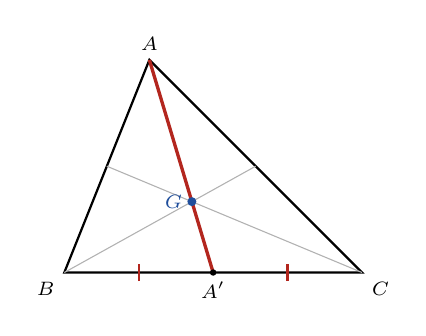
\begin{tikzpicture}[scale=0.9,font=\scriptsize]
\coordinate (A) at (1.2,3); \coordinate (B) at (0,0); \coordinate (C) at (4.2,0);
\draw[thick] (A)--(B)--(C)--cycle;
\node[above] at (A){$A$}; \node[below left] at (B){$B$}; \node[below right] at (C){$C$};
\draw[gray!60] (B)--(2.7,1.5); \draw[gray!60] (C)--(0.6,1.5);
\draw[cThm,very thick] (A)--(2.1,0);
\draw[cThm,thick] ($(1.05,0)+(0,-0.12)$)--($(1.05,0)+(0,0.12)$);\draw[cThm,thick] ($(3.15,0)+(0,-0.12)$)--($(3.15,0)+(0,0.12)$);
\fill (2.1,0) circle (1.3pt) node[below]{$A'$};
\fill[cDef] (1.8,1) circle (1.8pt) node[left,cDef]{$G$};
\end{tikzpicture}
\end{LTR}}
\end{BOX}
\begin{BOX}{cDef}{الارتفاع: «من رأس عمودياً على الضلع المقابل»}
\RL{0.55}{%
\textbf{الارتفاع المتعلق بالضلع $[BC]$} هو المستقيم الذي يشمل الرأس $A$ و\textbf{يعامد} $(BC)$ في النقطة $H_A$ (قدم الارتفاع).
\begin{itemize}
\item الطول $AH_A$ هو ارتفاع المثلث ، ونستعمله في المساحة: $S=\dfrac{BC\times AH_A}{2}$.
\item الارتفاعات الثلاثة تتلاقى في $H$ \textbf{المركز القائم}.
\item الارتفاع \textbf{لا يمر بالضرورة} بمنتصف الضلع.
\end{itemize}}{0.42}{%
\begin{LTR}\centering
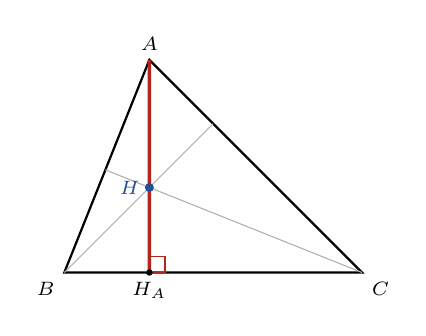
\begin{tikzpicture}[scale=0.9,font=\scriptsize]
\coordinate (A) at (1.2,3); \coordinate (B) at (0,0); \coordinate (C) at (4.2,0);
\draw[thick] (A)--(B)--(C)--cycle;
\node[above] at (A){$A$}; \node[below left] at (B){$B$}; \node[below right] at (C){$C$};
\draw[gray!60] (B)--($(A)!(B)!(C)$); \draw[gray!60] (C)--($(A)!(C)!(B)$);
\draw[cThm,very thick] (A)--(1.2,0);
\draw[cThm] (1.2,0)--++(0.22,0)--++(0,0.22)--++(-0.22,0);
\fill (1.2,0) circle (1.3pt) node[below]{$H_A$};
\fill[cDef] (1.2,1.2) circle (1.8pt) node[left,cDef]{$H$};
\end{tikzpicture}
\end{LTR}}
\end{BOX}
\begin{BOX}{cDef}{المنصف: «يقسم الزاوية نصفين»}
\RL{0.55}{%
\textbf{منصف الزاوية $\widehat A$} هو المستقيم الذي يقسمها إلى زاويتين \textbf{متقايستين} (القوسان الملونان).
\begin{itemize}
\item كل نقطة من المنصف \textbf{متساوية البعد} عن ضلعي الزاوية.
\item المنصفات الثلاثة تتلاقى في $I$ ، المتساوية البعد عن الأضلاع الثلاثة: الدائرة التي مركزها $I$ \textbf{تمس الأضلاع الثلاثة} (الدائرة المحاطة).
\end{itemize}}{0.42}{%
\begin{LTR}\centering
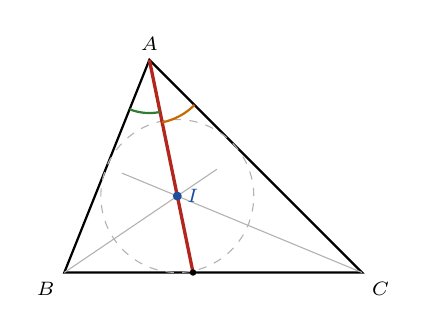
\begin{tikzpicture}[scale=0.9,font=\scriptsize]
\coordinate (A) at (1.2,3); \coordinate (B) at (0,0); \coordinate (C) at (4.2,0);
\draw[thick] (A)--(B)--(C)--cycle;
\node[above] at (A){$A$}; \node[below left] at (B){$B$}; \node[below right] at (C){$C$};
\draw[gray!60,dashed] (1.594,1.079) circle (1.079);
\draw[gray!60] (B)--($(B)!1.35!(1.594,1.079)$); \draw[gray!60] (C)--($(C)!1.3!(1.594,1.079)$);
\draw[cThm,very thick] (A)--(1.816,0);
\draw[cRem,thick] (A)++(-111.8:0.75) arc (-111.8:-78.4:0.75);
\draw[cEx,thick] (A)++(-78.4:0.9) arc (-78.4:-45:0.9);
\fill (1.816,0) circle (1.3pt);
\fill[cDef] (1.594,1.079) circle (1.8pt) node[right,cDef]{$I$};
\end{tikzpicture}
\end{LTR}}
\end{BOX}
\begin{molahada}[للتمييز بسرعة]
\renewcommand{\arraystretch}{1.4}
\centering
\begin{tabular}{|C|C|C|C|C|}\hline
\rowcolor{cDef!12}\textbf{المستقيم} & \textbf{يمر برأس؟} & \textbf{يمر بالمنتصف؟} & \textbf{يعامد الضلع؟} & \textbf{يقسم زاوية؟}\\\hline
\textbf{المحور} & ليس بالضرورة & نعم & نعم & لا\\\hline
\textbf{المتوسط} & نعم & نعم & ليس بالضرورة & لا\\\hline
\textbf{الارتفاع} & نعم & ليس بالضرورة & نعم & لا\\\hline
\textbf{المنصف} & نعم & ليس بالضرورة & ليس بالضرورة & نعم\\\hline
\end{tabular}
\end{molahada}
\begin{khassia}[مستقيم المنتصفين]
\RL{0.6}{%
في مثلث $ABC$:
\begin{itemize}
\item المستقيم الذي يشمل منتصفي ضلعين يوازي حامل الضلع الثالث ، و $IJ=\dfrac12BC$ ($I$ منتصف $[AB]$ و $J$ منتصف $[AC]$).
\item المستقيم الذي يشمل منتصف ضلع ويوازي حامل ضلع ثانٍ يقطع الضلع الثالث في منتصفه.
\end{itemize}}{0.37}{%
\begin{LTR}\centering
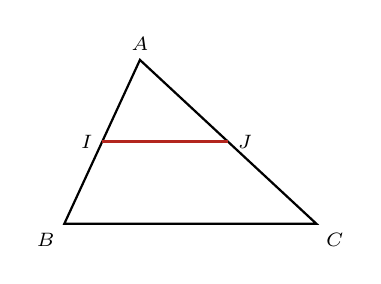
\begin{tikzpicture}[scale=0.8,font=\scriptsize]
\coordinate (A) at (1.2,2.6); \coordinate (B) at (0,0); \coordinate (C) at (4,0);
\draw[thick] (A)--(B)--(C)--cycle;
\draw[cThm,very thick] ($(A)!0.5!(B)$)--($(A)!0.5!(C)$);
\node[above] at (A){$A$}; \node[below left] at (B){$B$}; \node[below right] at (C){$C$};
\node[left] at ($(A)!0.5!(B)$){$I$}; \node[right] at ($(A)!0.5!(C)$){$J$};
\end{tikzpicture}
\end{LTR}}
\end{khassia}
\begin{khassia}[المثلث القائم والدائرة]
المثلث $ABC$ قائم في $A$ $\iff$ $A$ تنتمي إلى الدائرة التي قطرها $[BC]$. \ وطول المتوسط المتعلق بالوتر يساوي نصف الوتر: $AA'=\dfrac{BC}2$.
\end{khassia}

% =====================================================================
\section{مبرهنة فيثاغورس وعكسها}
\begin{khassia}
\RL{0.6}{%
\begin{itemize}
\item \textbf{المبرهنة:} إذا كان $ABC$ قائماً في $A$ فإن \bx{BC^2=AB^2+AC^2}.
\item \textbf{العكس:} إذا كان $BC^2=AB^2+AC^2$ فإن $ABC$ قائم في $A$.
\item \textbf{النتيجة:} إذا كان $BC^2\ne AB^2+AC^2$ (حيث $BC$ أطول ضلع) فإن المثلث ليس قائماً.
\end{itemize}}{0.37}{%
\begin{LTR}\centering
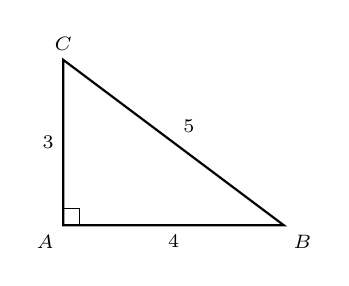
\begin{tikzpicture}[scale=0.7,font=\scriptsize]
\coordinate (A) at (0,0); \coordinate (B) at (4,0); \coordinate (C) at (0,3);
\draw[thick] (A)--(B)--(C)--cycle; \draw (0.3,0)--(0.3,0.3)--(0,0.3);
\node[below left] at (A){$A$}; \node[below right] at (B){$B$}; \node[above] at (C){$C$};
\node[below] at (2,0){$4$}; \node[left] at (0,1.5){$3$}; \node[above right] at (2,1.5){$5$};
\end{tikzpicture}
\end{LTR}}
\end{khassia}
\begin{mithal}
$AB=5$ ، $AC=12$ ، $BC=13$: \ $AB^2+AC^2=25+144=169=BC^2$ ، إذن $ABC$ \textbf{قائم في $A$}. \quad $EF=4$ ، $EG=5$ ، $FG=6$: $16+25=41\ne36$: \textbf{ليس قائماً}.
\end{mithal}

% =====================================================================
\section{مبرهنة طالس وعكسها}
\begin{khassia}
\RL{0.6}{%
$(BM)$ و $(CN)$ مستقيمان متقاطعان في $A$ ، حيث $M\in(AB)$ و $N\in(AC)$.
\begin{itemize}
\item \textbf{المبرهنة:} إذا كان $(MN)\parallel(BC)$ فإن: \ \bx{\dfrac{AM}{AB}=\dfrac{AN}{AC}=\dfrac{MN}{BC}}.
\item \textbf{العكس:} إذا كان $\dfrac{AM}{AB}=\dfrac{AN}{AC}$ ، وكانت النقط $A$ ، $M$ ، $B$ و $A$ ، $N$ ، $C$ بنفس الترتيب ، فإن $(MN)\parallel(BC)$.
\end{itemize}}{0.37}{%
\begin{LTR}\centering
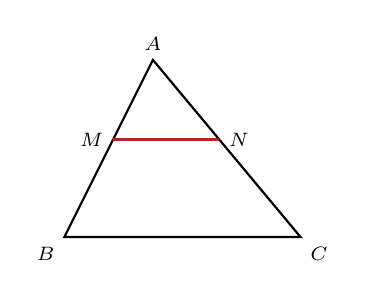
\begin{tikzpicture}[scale=0.75,font=\scriptsize]
\coordinate (A) at (0,3); \coordinate (B) at (-1.5,0); \coordinate (C) at (2.5,0);
\coordinate (M) at ($(A)!0.45!(B)$); \coordinate (N) at ($(A)!0.45!(C)$);
\draw[thick] (A)--(B)--(C)--cycle; \draw[cThm,very thick] (M)--(N);
\node[above] at (A){$A$}; \node[below left] at (B){$B$}; \node[below right] at (C){$C$};
\node[left] at (M){$M$}; \node[right] at (N){$N$};
\end{tikzpicture}
\end{LTR}}
\end{khassia}
\begin{mithal}
$AB=6$ ، $AM=2$ ، $AC=9$ و $(MN)\parallel(BC)$: \ $\dfrac{AN}{9}=\dfrac26$ ، إذن \bx{AN=3}. \ وإذا كان $BC=7{,}5$ فإن $MN=\dfrac13\times7{,}5=\bx{2{,}5}$.
\end{mithal}

% =====================================================================
\section{النسب المثلثية في مثلث قائم}
\begin{tarif}
\RL{0.6}{%
$ABC$ قائم في $A$ ، و $\widehat B$ زاوية حادة:
\[\cos\widehat B=\frac{AB}{BC}=\frac{\text{\ar{المجاور}}}{\text{\ar{الوتر}}}\qquad;\qquad\sin\widehat B=\frac{AC}{BC}=\frac{\text{\ar{المقابل}}}{\text{\ar{الوتر}}}\]
\[\tan\widehat B=\frac{AC}{AB}=\frac{\text{\ar{المقابل}}}{\text{\ar{المجاور}}}.\]
ومن أجل كل زاوية حادة $\alpha$: \ $\cos^2\alpha+\sin^2\alpha=1$ و $\tan\alpha=\dfrac{\sin\alpha}{\cos\alpha}$.}{0.37}{%
\begin{LTR}\centering
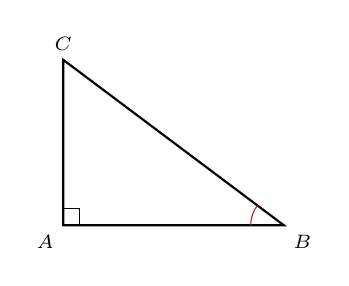
\begin{tikzpicture}[scale=0.7,font=\scriptsize]
\coordinate (A) at (0,0); \coordinate (B) at (4,0); \coordinate (C) at (0,3);
\draw[thick] (A)--(B)--(C)--cycle; \draw (0.3,0)--(0.3,0.3)--(0,0.3);
\draw[cThm] (3.4,0) arc (180:143:0.6);
\node[below left] at (A){$A$}; \node[below right] at (B){$B$}; \node[above] at (C){$C$};
\end{tikzpicture}
\end{LTR}}
\end{tarif}
\begin{mithal}
$ABC$ قائم في $A$ ، $BC=10$ و $\widehat B=30^\circ$: \ $AC=BC\sin30^\circ=\bx{5}$ ، و $AB=BC\cos30^\circ=10\times\dfrac{\sqrt3}2=\bx{5\sqrt3}$.
\end{mithal}

% =====================================================================
\section{المثلثات المتقايسة}
\begin{tarif}
نقول إن مثلثين \textbf{متقايسان} إذا كانت أضلاعهما متقايسة مثنى مثنى وزواياهما متقايسة مثنى مثنى (أي يمكن تطبيق أحدهما على الآخر).
\end{tarif}
\begin{khassia}[حالات التقايس]
يكون مثلثان متقايسين إذا تحقق أحد الشروط الثلاثة:
\begin{enumerate}
\item \textbf{(ض ، ض ، ض):} الأضلاع الثلاثة متقايسة مثنى مثنى.
\item \textbf{(ض ، ز ، ض):} ضلعان متقايسان والزاوية المحصورة بينهما متقايسة.
\item \textbf{(ز ، ض ، ز):} ضلع متقايس والزاويتان المجاورتان له متقايستان.
\end{enumerate}
\end{khassia}
\begin{mithal}
\RL{0.6}{%
$ABCD$ متوازي أضلاع مركزه $O$. \ المثلثان $OAB$ و $OCD$ متقايسان:\par
$OA=OC$ و $OB=OD$ (القطران متناصفان) ، و $\widehat{AOB}=\widehat{COD}$ (متقابلتان بالرأس): الحالة \textbf{(ض ، ز ، ض)}. \ ومنه $AB=CD$.}{0.37}{%
\begin{LTR}\centering
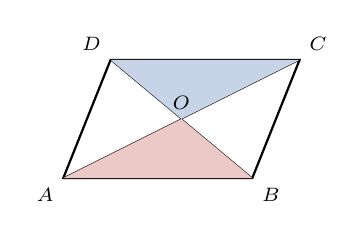
\begin{tikzpicture}[scale=0.6,font=\scriptsize]
\coordinate (A) at (0,0); \coordinate (B) at (4,0); \coordinate (C) at (5,2.5); \coordinate (D) at (1,2.5); \coordinate (O) at (2.5,1.25);
\draw[thick] (A)--(B)--(C)--(D)--cycle; \draw (A)--(C) (B)--(D);
\fill[cThm!25] (O)--(A)--(B)--cycle; \fill[cDef!25] (O)--(C)--(D)--cycle;
\node[below left] at (A){$A$}; \node[below right] at (B){$B$}; \node[above right] at (C){$C$}; \node[above left] at (D){$D$}; \node[above] at (O){$O$};
\end{tikzpicture}
\end{LTR}}
\end{mithal}

% =====================================================================
\section{المثلثات المتشابهة}
\begin{tarif}
نقول إن مثلثين \textbf{متشابهان} إذا كانت زواياهما متقايسة مثنى مثنى. \ عندئذ أطوال أضلاع أحدهما متناسبة مع أطوال أضلاع الآخر:
\[\frac{A'B'}{AB}=\frac{B'C'}{BC}=\frac{A'C'}{AC}=k\qquad(k\ \text{\ar{نسبة التشابه}}).\]
\end{tarif}
\begin{khassia}[حالات التشابه]
يكون مثلثان متشابهين إذا تحقق أحد الشروط:
\begin{enumerate}
\item لهما \textbf{زاويتان} متقايستان مثنى مثنى.
\item أطوال أضلاعهما \textbf{متناسبة}.
\item لهما زاوية متقايسة ، وطولا الضلعين المحصورين بها متناسبان.
\end{enumerate}
\end{khassia}
\begin{khassia}[المساحات]
إذا كان مثلثان متشابهين بنسبة $k$ (المثلث الثاني تكبير أو تصغير للأول) فإن: \ \bx{S'=k^2\times S}.
\end{khassia}
\begin{mithal}
\RL{0.6}{%
$ABC$ مثلث ، $M\in[AB]$ و $N\in[AC]$ حيث $(MN)\parallel(BC)$ ، $AM=2$ و $AB=5$.\par
المثلثان $AMN$ و $ABC$ متشابهان (لهما الزاوية $\widehat A$ مشتركة ، و $\widehat{AMN}=\widehat{ABC}$ بالتماثل) ، ونسبة التشابه $k=\dfrac25$.\par
إذا كانت مساحة $ABC$ هي $50\,cm^2$ فإن مساحة $AMN$ هي $\Big(\dfrac25\Big)^2\times50=\bx{8\,cm^2}$.}{0.37}{%
\begin{LTR}\centering
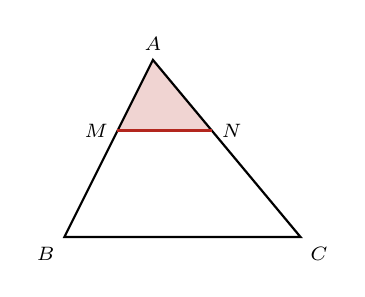
\begin{tikzpicture}[scale=0.75,font=\scriptsize]
\coordinate (A) at (0,3); \coordinate (B) at (-1.5,0); \coordinate (C) at (2.5,0);
\coordinate (M) at ($(A)!0.4!(B)$); \coordinate (N) at ($(A)!0.4!(C)$);
\fill[cThm!20] (A)--(M)--(N)--cycle;
\draw[thick] (A)--(B)--(C)--cycle; \draw[cThm,very thick] (M)--(N);
\node[above] at (A){$A$}; \node[below left] at (B){$B$}; \node[below right] at (C){$C$};
\node[left] at (M){$M$}; \node[right] at (N){$N$};
\end{tikzpicture}
\end{LTR}}
\end{mithal}

% =====================================================================
\section{التحويلات النقطية في المستوي}
\begin{tarif}
\begin{itemize}
\item \textbf{الانسحاب} الذي شعاعه $\vec u$: يرفق بكل نقطة $M$ النقطة $M'$ حيث \bx{\V{MM'}=\vec u}.
\item \textbf{التناظر المركزي} الذي مركزه $O$: $M'$ هي النقطة حيث $O$ منتصف $[MM']$ ، أي \bx{\V{OM'}=-\V{OM}}.
\item \textbf{التناظر المحوري} الذي محوره $(\Delta)$: $M'$ هي النقطة حيث $(\Delta)$ محور القطعة $[MM']$ (إذا كان $M\notin(\Delta)$) ، و $M'=M$ إذا كان $M\in(\Delta)$.
\item \textbf{الدوران} الذي مركزه $O$ وزاويته $\theta$: $M'$ هي النقطة حيث \bx{OM'=OM} و $\big(\V{OM};\V{OM'}\big)=\theta$ (في الاتجاه المباشر إذا كان $\theta>0$).
\end{itemize}
\end{tarif}
\begin{LTR}
\begin{center}
\begin{tikzpicture}[scale=0.6,font=\scriptsize]
\begin{scope}[xshift=17.5cm]
\draw[thick] (0,0)--(1.5,0)--(0.4,1.2)--cycle; \draw[cThm,thick] (2.5,0.8)--(4,0.8)--(2.9,2)--cycle;
\draw[cRem,very thick,-{Stealth}] (0.5,-0.4)--(3,0.4) node[midway,below right]{$\vec u$};
\node at (2,-1.2){\foreignlanguage{arabic}{انسحاب}};
\end{scope}
\begin{scope}[xshift=12cm]
\fill (1.5,0.8) circle (2pt) node[below]{$O$};
\draw[thick] (0,0)--(1,0)--(0.2,1)--cycle; \draw[cThm,thick] (3,1.6)--(2,1.6)--(2.8,0.6)--cycle;
\draw[gray,dashed] (0,0)--(3,1.6);
\node at (1.5,-1.2){\foreignlanguage{arabic}{تناظر مركزي}};
\end{scope}
\begin{scope}[xshift=6.5cm]
\draw[cRem,thick] (1.5,-0.6)--(1.5,2.2) node[above]{$(\Delta)$};
\draw[thick] (0,0)--(1,0.2)--(0.3,1.3)--cycle; \draw[cThm,thick] (3,0)--(2,0.2)--(2.7,1.3)--cycle;
\node at (1.5,-1.2){\foreignlanguage{arabic}{تناظر محوري}};
\end{scope}
\begin{scope}[xshift=0.5cm]
\fill (0,0) circle (2pt) node[below left]{$O$};
\draw[thick] (1.5,0)--(2.5,0)--(2,0.8)--cycle;
\draw[cThm,thick,rotate=90] (1.5,0)--(2.5,0)--(2,0.8)--cycle;
\draw[cRem,->] (1.2,0) arc (0:90:1.2) node[midway,above right]{$\theta$};
\node at (1,-1.2){\foreignlanguage{arabic}{دوران}};
\end{scope}
\end{tikzpicture}
\end{center}
\end{LTR}
\begin{khassia}[خواص مشتركة: التحويلات تقايسات]
الانسحاب ، التناظر المركزي ، التناظر المحوري والدوران \textbf{تحافظ على}:
\begin{itemize}
\item \textbf{المسافات} (الأطوال) ، و\textbf{أقياس الزوايا} الهندسية ، و\textbf{المساحات}.
\item \textbf{الاستقامية} والمنتصف ، و\textbf{التوازي} و\textbf{التعامد}.
\end{itemize}
صورة مستقيم مستقيم ، صورة قطعة قطعة تقايسها ، صورة دائرة دائرة لها نفس نصف القطر ومركزها صورة المركز ، وصورة مثلث مثلث يقايسه.
\end{khassia}
\begin{molahada}
\begin{itemize}
\item صورة مستقيم بانسحاب أو بتناظر مركزي هو \textbf{مستقيم يوازيه}.
\item التناظر المركزي هو دوران زاويته $\pi$ (أي $180^\circ$).
\item الانسحاب والتناظر المركزي والدوران تحافظ على \textbf{اتجاه} الزوايا ، أما التناظر المحوري فيعكسه.
\end{itemize}
\end{molahada}

% =====================================================================
\section{تمرين محلول وخلاصة الطرائق}
\begin{tmr}
$ABC$ مثلث قائم في $A$ حيث $AB=6$ و $AC=8$. \ $I$ منتصف $[BC]$ ، و $M$ نقطة من $[AB]$ حيث $AM=1{,}5$ ، والمستقيم الذي يشمل $M$ ويوازي $(BC)$ يقطع $[AC]$ في $N$.
\begin{enumerate}
\item احسب $BC$ ثم $AI$.
\item احسب $AN$ و $MN$.
\item احسب $\cos\widehat{ABC}$ و $\tan\widehat{ABC}$.
\item لتكن $D$ صورة $A$ بالتناظر الذي مركزه $I$. ما طبيعة الرباعي $ABDC$؟
\end{enumerate}
\end{tmr}
\begin{hal}
\textbf{1.} فيثاغورس: $BC^2=36+64=100$ ، \bx{BC=10}. \ $[AI]$ متوسط متعلق بالوتر: \bx{AI=\dfrac{BC}2=5}.
\QQ{2} طالس ($(MN)\parallel(BC)$): $\dfrac{AM}{AB}=\dfrac{1{,}5}{6}=\dfrac14$ ، إذن $AN=\dfrac14\times8=\bx{2}$ و $MN=\dfrac14\times10=\bx{2{,}5}$.
\QQ{3} $\cos\widehat B=\dfrac{AB}{BC}=\dfrac6{10}=\bx{0{,}6}$ ، و $\tan\widehat B=\dfrac{AC}{AB}=\dfrac86=\bx{\dfrac43}$.
\QQ{4} $I$ منتصف $[BC]$ و $[AD]$: القطران متناصفان ، فـ $ABDC$ متوازي أضلاع ، وفيه زاوية قائمة في $A$: \ \textbf{$ABDC$ مستطيل}.
\end{hal}
\begin{BOX}{cMeth}{ماذا أفعل عندما يُطلب مني $\ldots$؟}
\renewcommand{\arraystretch}{1.5}
\centering
\begin{tabular}{|p{0.56\textwidth}|p{0.32\textwidth}|}\hline
\cellcolor{cMeth!15}\textbf{الطريقة} & \cellcolor{cMeth!15}\textbf{المطلوب}\\\hline
فيثاغورس في مثلث قائم ، أو طالس مع التوازي ، أو النسب المثلثية. & حساب طول\\\hline
عكس فيثاغورس ، أو نقطة على دائرة قطرها الوتر. & إثبات أن مثلثاً قائم\\\hline
عكس طالس ، أو مستقيم المنتصفين. & إثبات توازي مستقيمين\\\hline
إحدى الحالات الثلاث (ض ض ض) ، (ض ز ض) ، (ز ض ز). & إثبات تقايس مثلثين\\\hline
زاويتان متقايستان ، أو أضلاع متناسبة. & إثبات تشابه مثلثين\\\hline
نسبة التشابه $k$ ثم $S'=k^2S$. & مساحة مثلث مشابه\\\hline
نستعمل أن التحويل يحافظ على الأطوال والزوايا والتوازي. & خواص صورة شكل بتحويل\\\hline
\end{tabular}
\end{BOX}

\end{document}
